\documentclass[parskip]{report}
\usepackage[utf8]{inputenc}
\usepackage[]{amsmath}
\usepackage[]{amssymb}
\usepackage[]{setspace}
\usepackage[]{tikz}
\usepackage[]{xcolor}
\usepackage[]{enumitem}
\usepackage{titlesec}
\usepackage{geometry}

\geometry{letterpaper, portrait, margin=1in}

\usetikzlibrary{positioning}
\usetikzlibrary{fit}

\onehalfspacing
\setlength{\parskip}{1em}
\setlength{\parindent}{0pt}
\setlist[enumerate]{label = \textbf{\alph*.}}


\newenvironment{q}
    {\begin{bfseries}}
    {\end{bfseries}}

\newenvironment{ans}
    {\begin{text}{\textbf{Answer:}}}
    {\end{text}}

\newenvironment{prf}
    {\begin{text}{\textbf{Proof:}}}
    {\end{text}}

\newenvironment{xx}
    {
        \color{red}
        \begin{text}
            {\textbf{Scratchpad:}}
    }
    {
        \end{text}
    }

% \courselabel{Analysis I}
% \student{Rachel Shu}
% \exercisesheet{Chapter 3.3}{Functions}
% \school{Analysis I}
% \semester{}
% \university{}
\date{April 27, 2023}

\renewcommand{\thesection}{Section \arabic{chapter}.\arabic{section}}
\titleformat{\section}{\normalfont\fontsize{18}{18}\bfseries}{\thesection}{1em}{}

\renewcommand{\thesubsection}{Exercise \arabic{chapter}.\arabic{section}.\arabic{subsection}}
\titleformat{\subsection}{\normalfont\fontsize{15}{15}\bfseries}{\thesubsection}{1em}{}

\begin{document}

\setcounter{chapter}{3}

\setcounter{section}{2}
\section{Functions}

\setcounter{subsection}{1}
\subsection{}

\begin{q}
Let $f : X \to Y$ and $g : Y \to Z$ be functions. Show that if $f$ and $g$ are both injective, then so is $g \circ f$; similarly show that if $f$ and $g$ are both surjective, then so is $g \circ f$.
\end{q}


\begin{prf}
    Suppose $f$ and $g$ are injective.
    We need to show that for each $x$ and $x'$ in $X$, $x \neq x'$ implies $(g \circ f)(x) \neq (g \circ f)(x')$.
    The assumption that $f$ is injective tells us that for every $x$ and $x'$ in $X$, $x \neq x' \implies f(x) \neq f(x')$.
    Since each $f(x)$ and $f(x')$ is in $Y$, the assumption that $g$ is injective also tells us that for every $f(x)$ and $f(x')$ in $Y$, $f(x) \neq f(x') \implies g(f(x)) \neq g(f(x'))$.
    Thus for each $x$ and $x'$ in $X$, $x \neq x'$ implies $(g \circ f)(x) \neq (g \circ f)(x')$ as desired.
    
    Now suppose $f$ and $g$ are surjective.
    We need to show that for each $z$ in $Z$, there exists $x$ in $X$ such that $(g \circ f)(x)=z$.
    The assumption that $f$ is surjective tells us that for each $y$ in $Y$, there exists $x$ in $X$ such that $f(x)=y$.
    Since each $f(x)$ is in $Y$, the assumption that $g$ is surjective tells us that for each $z$ in $Z$, there exists $f(x)$ in $Y$, and thus $x$ in $X$, such that $g(f(x))=z$. Then for each $z$ in $Z$, there exists $x$ in $X$ such that $(g \circ f)(x)=z$, as desired. $\square$
\end{prf}

\subsection{}
\begin{q}
    When is the empty function into a given set injective? surjective? bijective?
\end{q}

\begin{ans}
    The empty function is only bijective into the empty set.
\end{ans}

\begin{prf}
    For the empty function to be injective into a given set, for each $x$ and $x'$ in $\emptyset$, $x \neq x'$ implies $empty(x) \neq empty(x')$.
    This is vacuously true as neither $x$ nor $x'$ exist.
    Thus the empty function is injective into all sets.
    
    For the empty function to be surjective onto a given set, for each $y$ in some set $Y$ there needs to be some $x$ in $\emptyset$ such that $empty(x)=y$.
    But there are no $x$ in $\emptyset$, so this is false if there are any $y$ in $Y$.
    Thus the empty function is only surjective onto the empty set, when it is vacuously true.
    
    For the empty function to be bijective into a given set, it must be injective into and surjective onto that set. Since the empty function is only surjective onto the empty set, it is only bijective into the empty set.
    $\square$
\end{prf}

\stepcounter{subsection}
\subsection{}
\begin{q}
Let $f: X \to Y$ and $g: Y \to Z$ be functions.
\end{q}

\begin{enumerate}
    \item
    \begin{q}
        Show that if $g \circ f$ is injective, then $f$ must be injective.
    \end{q}

    \begin{prf}
        For the sake of contradiction suppose $g \circ f$ is injective but $f$ is not.
        Then there exists some $x$ and $x'$ in $X$ that go to the same $y$ in $Y$.
        By the definition of a function, when we apply $g$ each $y$ in Y goes to exactly one $z$ in Z, so when we apply $g \circ f$, any $x$ and $x'$ that go to the same $y$ go to the same $z$, which contradicts the assumption that $g \circ f$ is injective.
        Thus if $g \circ f$ is injective $f$ must also be.
        $\square$
    \end{prf}

    \item
    \begin{q}
        Is it true that $g$ must also be injective?
    \end{q}

   \begin{ans}
     No.
   \end{ans}

    \begin{prf}
        A counterexample shows that $g$ is not necessarily injective when $(g \circ f)$ is.
        Suppose $X$ is the empty set, $Y$ is $\mathbb{N}$, $Z$ is $\mathbb{N}$, and suppose $g$ is the function $x \mapsto 0$.
        We can see $g$ is not injective from $Y$ to $Z$. (To pick one counterexample, $g(1)$ and $g(2)$ are equal.)
        But since any function from $\emptyset$ is an empty function, which is injective, $(g \circ f)(x)$ is injective.
        $\square$
    \end{prf}

    \item
    \begin{q}
        Show that if $g \circ f$ is surjective, then $g$ must be surjective.
    \end{q}

    \begin{prf}
        For the sake of contradiction, suppose $g \circ f$ is surjective but $g$ is not.
        If $g$ is not surjective, there exists some $z$ in $Z$ for which there is no $y$ in $Y$ such that $g(y)=z$.
        Then as all $f(x)$ are in $Y$ there is also no $f(x)$ such that $g(f(x))=z$.
        By the definition of a function if $f(x)$ does not exist then $x$ cannot exist.
        So there is some $z$ in $Z$ for which there is no $x$ in $x$ such that $g(f(x))=z$.
        But this contradicts our supposition that $g \circ f$ is surjective.
        Thus if $g \circ f$ is surjective then $g$ is too.
        $\square$
    \end{prf}

    \item
    \begin{q}
        Is it true that $f$ must also be surjective?
    \end{q}

    \begin{ans}
        No.
    \end{ans}

    % (informal) A function g(y) can still be surjective even if multiple inputs go to the same output. if for each output, at least one input's input exists, then g(f(x)) is true. but the other inputs might not have inputs, so f(x) is not necessarily true (and I don't know what to do with not necessarily true cases).

    \begin{prf}
    To provide a counterexample, let $g: Y \to Z$ be a function which is surjective but for which there is some $y \in Y$ and some $y' \in Y$ such that for some $z'$ in $Z$, $z'=g(y)=g(y')$, i.e. $g$ is not injective.
    Also let $f: X \to Y$ be a function for which there is some $x$ such that $f(x)=y$ for all $y \in Y$ except $y'$, in which case $f$ is not surjective (but would be if $y'$ were left out).
    See the diagram below for one example of such a function:

    \begin{center}
    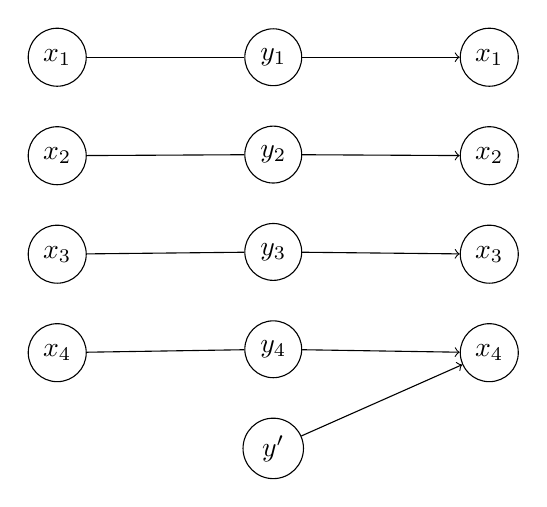
\begin{tikzpicture}[
        align=center,
        head/.style = {node distance=.25cm and 2cm, draw, circle},
        main/.style = {node distance=.5cm and 2cm, draw, circle}
    ]

        \node[main] (x1) {$x_1$};
        \node[main] (x2) [below=of x1] {$x_2$};
        \node[main] (x3) [below=of x2] {$x_3$};
        \node[main] (x4) [below=of x3] {$x_4$};
        \node[main] (y1) [right=of x1] {$y_1$};
        \node[main] (y2) [below=of y1] {$y_2$};
        \node[main] (y3) [below=of y2] {$y_3$};
        \node[main] (y4) [below=of y3] {$y_4$};
        \node[main] (y') [below=of y4] {$y'$};
        \node[main] (z1) [right=of y1] {$x_1$};
        \node[main] (z2) [below=of z1] {$x_2$};
        \node[main] (z3) [below=of z2] {$x_3$};
        \node[main] (z4) [below=of z3] {$x_4$};

        \draw[->] (x1) -- (y1) -- (z1);
        \draw[->] (x2) -- (y2) -- (z2);
        \draw[->] (x3) -- (y3) -- (z3);
        \draw[->] (x4) -- (y4) -- (z4);
        \draw[->] (y') -- (z4);

    \end{tikzpicture}
    \end{center}

    We can verify that $(g \circ f)$ is still surjective, since for each $z$ in $Z$ there is at least one $f(x)$ such that $g(f(x))=z$.
    In particular, for the $z'$ which is equal to $g(y')$, since it is also equal to $g(y)$, and $f(x)=y$ for all $y \in Y$ except $y'$, there is some $x$ for which $(g \circ f)(x)=z'$.

    Thus it is not the case that if $f$ is not surjective that $(g \circ f)$ is also not, or to remove the contrapositive, it is not the case that if $(g \circ f)$ is surjective that $f$ is also.
    $\square$
\end{prf}
\end{enumerate}

\addtocounter{subsection}{2}
\subsection{}

\begin{q}
    If $X$ is a subset of $Y$, let $\iota_{X\to Y} : X \to Y$ be \emph{the inclusion map from $X$ to $Y$}, defined by mapping $x \mapsto x$ for all $x \in X$, i.e., $\iota_{X\to Y}(x) := x$ for all $x \in X$.
    The map $\iota_{X\to X}$ is in particular called the \emph{identity map} on $X$.
\end{q}
\begin{enumerate}
    \item
    \begin{q}
        If $X \subseteq Y \subseteq Z$ then $\iota_{Y\to Z} \circ \iota_{X\to Y} = \iota_{X\to Z}$.
    \end{q}

    \begin{prf}
        To prove equality, we need to show the domains and codomains of $\iota_{Y\to Z} \circ \iota_{X\to Y}$ and $\iota_{X\to Z}$ agree, and that for all $x$ in their common domain $\iota_{Y\to Z} \circ \iota_{X\to Y}(x) = \iota_{X\to Z}(x)$.

        Let $X \subseteq Y \subseteq Z$. Since $X \subseteq Y$, $\iota_{X\to Y}: X \to Y$ and since $Y \subseteq Z$, $\iota_{Y\to Z}: Y \to Z$, by the definition of composition (Definition 3.3.13) $\iota_{Y\to Z} \circ \iota_{X\to Y}: X \to Z$. Likewise, since $X \subseteq Z$, $\iota_{X\to Z}: X \to Z$, thus the codomains of the two functions agree.

        Since $Y \subseteq Z$, we know $\iota_{Y\to Z}(y) := y$ for all $y \in Y$.
        In particular, since $X \subseteq Y$, $\iota_{Y\to Z}(\iota_{X\to Y}(x)) := \iota_{X\to Y}(x)$, which is $x$ for all $X$.
        Likewise, since $X \subseteq Z$, $\iota_{X\to Z}(x) := x$ for all $X$.Thus for all $x \in X$, the output of $\iota_{Y\to Z}(\iota_{X\to Y}(x))$ is equal to the output of $\iota_{X\to Z}(x)$.

        Therefore the two functions are equal.
        $\square$
    \end{prf}

    \item 
    \begin{q}
        Show that if $f: A \to B$ is any function, then $f = f \circ \iota_{A \to A} = \iota_{B \to B} \circ f$.
    \end{q}

    \begin{prf}
        To prove equality, we need to show the domains and codomains of $f$, $f \circ \iota_{A \to A}$, and $\iota_{B \to B} \circ f$ all agree, and that for all $x$ in their common domain, $f(x) = f \circ \iota_{A \to A}(x) = \iota_{B \to B} \circ f(x)$.

        Let $f: A \to B$ be any function from $A$ to $B$.
        Since $A \subseteq A$, we are given $\iota_{A \to A}: A \to A$.
        Then by the function composition rule (Definition 3.3.13) $f \circ \iota_{A\to A}: A \to B$ as well.
        Likewise, since $B \subseteq B$, we are given $\iota_{B \to B}: A \to B$.
        So composing $\iota_{B\to B} \circ f$ gives us a signature of $A \to B$ once again.
        Thus the domains and codomains all agree.

        We now only need the outputs are equal. Since $f: A \to B$, for every element $a \in A$, for some element $b \in B$ we have $f(a)=b$.

        Since $A \subseteq A$, for each element $a \in A$, we have $\iota_{A\to A}(a)$ = $a$.
        So the function $(f \circ \iota_{A \to A}): A \to B$ first sends each $a$ to itself, then each $a$ to $b$.
        Thus for every element $a \in A$, for some element $b \in B$ we again have $(f \circ \iota_{A \to A})(a)=b$.

        Likewise, since $B \subseteq B$, for each element $b \in B$, we have $\iota_{B\to B}(b)$ = $b$.
        So the function $\iota_{B \to B} \circ f.$ first sends each $a$ to $b$, then each $b$ to itself.
        Thus for every element $a \in A$, for some element $b \in B$ we yet again have $\iota_{B \to B} \circ f(a)=b$.

        Thus the outputs are all equal, and the two functions are equal.
        $\square$
    \end{prf}

    \item 
    \begin{q}
        Show that if $f: A \to B$ is a bijective function, then $f \circ f^{-1} = \iota_{B \to B}$ and $f^{-1} \circ f = \iota_{A \to A}$.
    \end{q}

    \begin{prf}
        The axiom of set equality states that
        \begin{equation*}
                f: X \to Y
                =
                g: X' \to Y'
            \iff
            \biggl(
                X=X' \quad
                Y=Y' \quad
                \forall x \in X \;
                    f(x)=g(x)
            \biggr)
        \end{equation*}

        Let $f: A \to B$ be a bijective function, which by Remark 3.3.27 has an inverse function denoted $f^{-1}: B \to A$.
        We separate the claims by conjunction elimination, and first prove $f \circ f^{-1} = \iota_{B \to B}$.

        By the function composition rule (Definition 3.3.13), $f \circ f^{-1}$ is a function from $B \to B$. Since by definition $\iota_{B \to B}$ is from $B \to B$ as well, their domains and codomains agree.

        Since $f$ is bijective, for all $a \in A$, there exists exactly one $b \in B$ such that $f \; a \mapsto b$. We defined $f^{-1}$ as the function $b \mapsto a$. Then $f \circ f^{-1}$ is the function $(b \mapsto a) \mapsto b$, in other words $f \circ f^{-1}(b)=b$. We also know $\iota_{B \to B}(b)=b$. Thus $f \circ f^{-1} = \iota_{B \to B}$.

        The other part is very similar. $f^{-1} \circ f$ is a function from $A \to A$, which we also know is true of $\iota_{A \to A}$. Then $f^{-1} \circ f$ is the function $(a \mapsto b) \mapsto a$,in other words $f^{-1} \circ f(a)=a$. Likewise $\iota_{A \to A}(a)=a$. Thus $f^{-1} \circ f = \iota_{A \to A}$, and we have completed our proof.
        $\square$
    \end{prf}

    \item 
    \begin{q}
        Show that if $X$ and $Y$ are disjoint sets, and $f: X \to Z$ and $g: Y \to Z$ are functions, then there is a unique function $h: X \cup Y \to Z$ such that $h \circ \iota_{X \to X \cup Y} = f$ and $h \circ \iota_{Y \to X \cup Y} = g.$
    \end{q}

    
    \begin{prf}
        Let $X$ and $Y$ be disjoint sets, and $f: X \to Z$ and $g: Y \to Z$ be functions.
        We need to show that there is some function $h: X \cup Y \to Z$ which satisfies $h \circ \iota_{X \to X \cup Y} = f$ and $h \circ \iota_{Y \to X \cup Y} = g$, and then show that it is unique.
    
        By pairwise union, (Axiom 3.5) there exists $X \cup Y$. By the definition of disjunction, $X$ and $Y$ have no common elements, so $a \in X \cup Y$ is exclusively in $X$ xor $Y$. Thus we can construct the following:
    
        Let $h: X \cup Y \to Z$ = \(
            \begin{cases}
                f(a) & \text{if } a \in X \\
                g(a) & \text{if } a \in Y
            \end{cases}
        \)
        \\
    
        Using this $h$, suppose $h \circ \iota_{X \to X \cup Y}$.
        Since $h: X \cup Y \to Z$ and $\iota_{X \to X \cup Y}: X \to X \cup Y$, their composition $h \circ \iota_{X \to X \cup Y}$ is a function from $X \to Z$. 
        Thus it has the same type as $f$.
        For all $x \in X$, $\iota_{X \to X \cup Y}(x)=x$.
        This means $h \circ \iota_{X \to X \cup Y}(x) = h(x)$. Since $x$ in $X$, $h(x) = f(x)$.
        Therefore we have satisfied both conditions to prove $h \circ \iota_X \to X \cup Y = f$.

        Likewise, suppose $h \circ \iota_{Y \to X \cup Y}$.
        Since $h: X \cup Y \to Z$ and $\iota_{Y \to X \cup Y}: Y \to X \cup Y$, their composition $h \circ \iota_{Y \to X \cup Y}$ is a function from $Y \to Z$. 
        Thus it has the same type as $g$.
        For all $y \in Y$, $\iota_{Y \to X \cup Y}(y)=y$.
        This means $h \circ \iota_{Y \to X \cup Y}(y) = h(y)$. Since $y$ in $Y$, $h(y) = g(y)$.
        Now we have also satisfied both conditions to prove $h \circ \iota_X \to X \cup Y = g$.
    \end{prf}

    \begin{xx}
        We now prove uniqueness by contradiction.
        Suppose $h: X \cup Y \to Z$ is not unique.
        Then there exists some $h': X \cup Y \to Z$ such that $h \neq h'$ and yet both $h' \circ \iota_{X \to X \cup Y} = f$ and $h' \circ \iota_{Y \to X \cup Y} = g$ as well.
        We know that the domains and codomains are the same.
        hmm this seems wrong.
    \end{xx}


    \item \begin{q}
        Show that the hypothesis that $X$ and $Y$ are disjoint can be dropped in (d) if one adds the additional hypothesis that $f(x) = g(x)$ for all $x \in X \cap Y$.
    \end{q}

    \begin{prf}
        
    \end{prf}

    \begin{xx}
        
    \end{xx}

\end{enumerate}
        
\end{document}